% ******************************* Thesis Appendix B ********************************
\chapter{\mindphistar requirement in the signal region}
\label{ch:app_dphistar}

As described in chapter~\ref{ch:5}, an event level requirement is made in the
signal region such that all events have \mindphistar > 0.3, in order to remove
any remaining QCD MJ contamination. 
% This appendix outlines some of
% the studies used to motivate this requirement and characterises it's effect on
% the analysis.

% \section{Motivation}

% The hadronic signal region selection criteria are specifically
% designed to remove many orders of magnitude of QCD MJ events, in particular
% through the use of variables such as \alphat and \mhtmet.
% However, despite these strict requirements a small fraction of QCD MC events are
% observed to still pass the selection criteria.

% \begin{figure}[h!]
%   \centering
%   \begin{subfigure}[b]{0.46\textwidth}
%     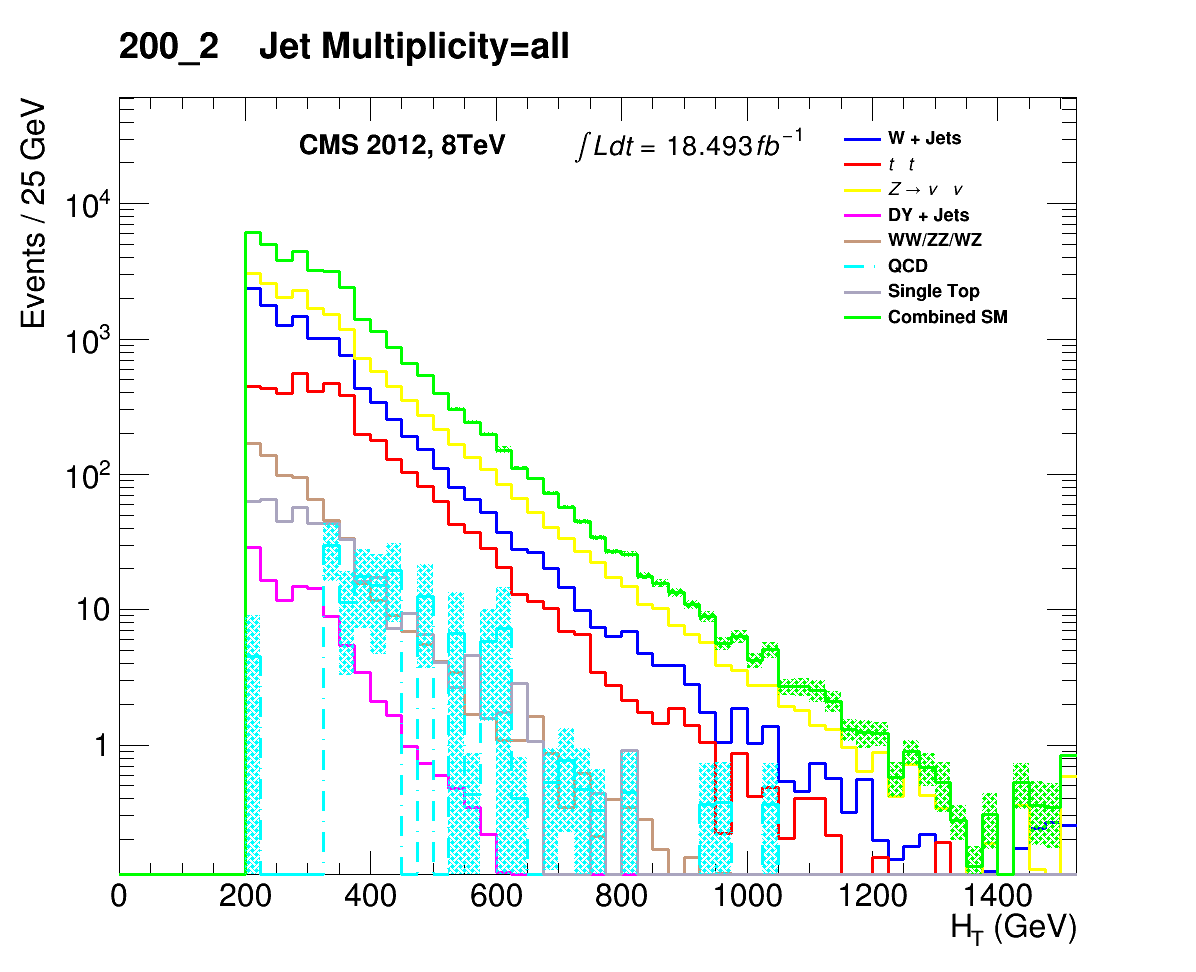
\includegraphics[width=\textwidth]{Figs/datamc/had/qcd/HT_all_200_upwards.png}
%     \caption{\HT}
%     \label{fig:had_qcd_mc_HT}
%   \end{subfigure}
%   \begin{subfigure}[b]{0.46\textwidth}
%     \includegraphics[width=\textwidth]
%     {Figs/datamc/had/qcd/JetMultiplicity_all_200_upwards.png}
%     \caption{\nj}
%     \label{fig:had_qcd_mc_njet}
%   \end{subfigure}\\
%   \begin{subfigure}[b]{0.46\textwidth}
%     \includegraphics[width=\textwidth]
%     {Figs/datamc/had/qcd/MET_all_200_upwards.png}
%     \caption{\met}
%     \label{fig:had_qcd_mc_met}
%   \end{subfigure}
%   \begin{subfigure}[b]{0.46\textwidth}
%     \includegraphics[width=\textwidth]
%     {Figs/datamc/had/qcd/MHTovMET_all_200_upwards.png}
%     \caption{\mhtmet}
%     \label{fig:had_qcd_mc_MHTMET}
%   \end{subfigure}
%   \caption{Distributions of various event level quantities for simulated MC
%   events split by physics process, with QCD shown in cyan. Plots shown are for
%   a fully inclusive selection of $\nj\geq2$, $\nb=0$ and $\HT>200\gev$.}
%   \label{fig:had_qcd_mc_distros}
% \end{figure}

% These remaining QCD events appear to originate from genuine physics processes,
% when a jet overlaps with genuine \met. This missing energy occurs due to heavy
% flavour mesons decaying leptonically. Of the lepton and neutrino pair produced,
% the neutrino
% carries the bulk share of the pair's momentum, leading to soft leptons which
% can evade leptonic vetoes and significant amounts of invisible energy. Similarly,
% as these leptons will be along the jet axis and in high-multiplicity events,
% it becomes increasingly likely for them to fail isolation requirements, and
% therefore not be considered by the leptonic vetoes.

\section{Simulation}
An event display of a typical event is shown in figure~\ref{fig:event_display_QCD}.
It is important to note the high amount, 185 \gev, of generator level
\met (`genmetP4True', thin pink arrow) pointing along the axis of a reconstructed
jet with $\Pt = 119 \gev$ (bold blue arrow) - a configuration which,
coupled with multiple additional jets, can conspire to give
large values of \alphat. The sum of the generator level \met and
the \Pt of the jet sum to the \Pt of the generator level jet (bold black arrow),
indicating that the missing energy of the event comes almost entirely from the
neutrinos from the decay of the jet. Furthermore, this implies the ratio
\mhtmet to be near unity, therefore allowing events to also evade the \mhtmet <
1.25 requirement of the signal region.

% \section{Isolating these events}

% It is possible to isolate these events used the \mindphistar variable described
% in section~\ref{sec:selec_crit}.

% \begin{figure}[h!]
% \centering
% \includegraphics[width=0.7\textwidth]
% {Figs/datapred/Prediction_ComMinBiasDPhi_acceptedJets_all_375_upwards_QCD.pdf}
% \label{fig:data_pred_dphistar_qcd}
% \caption{Data (black points) against the EWK background prediction 
% (stacked, yellow and purple) as a function of \mindphistar. The expected yield
% from QCD MC (cyan) is stacked on top of the EWK prediction. The plot represents
% the hadronic signal selection with a fully inclusive selection, $\nb \geq 0$,
% $\nj \geq 2$ and $\HT > 375 \gev$.}
% \end{figure}

% Figure~\ref{fig:data_pred_dphistar_qcd} shows the data observation in the
% hadronic region and the EWK background prediction prediction from the \mj and 
% \mmj control samples only, made using the transfer factor technique as a
% function of the \mindphistar variable. Furthermore, the observed yield from QCD
% MC is shown in cyan, stacked on top of the EWK prediction. The excess of events
% observed at low \mindphistar in data over the EWK prediction is accounted for by
% the QCD MC yields.

% An additional requirement of \mindphistar > 0.3 in the signal
% region removes this additional background source, such that any remaining
% contamination is considered entirely negligible with respect to the EWK
% background prediction.


% \section{Effect of hadronic region}

% \emph{How well does this work?} Very well! Removes all remaining QCD events that
% contain missing energy. \emph{What about the remaining few QCD MG events at high
% dPhiStar?} can show rob's plots of the dphiStar above/below

\section{Effect on signal models}
The effect of the \mindphistar > 0.3 requirement on the \texttt{T2cc} and
\texttt{T2degen} signal models is shown in figures~\ref{fig:t2cc_dphistar_effchange}
and \ref{fig:t2degen_dphistar_effchange} respectively.

\begin{figure}[h!]
  \centering
  \begin{subfigure}[b]{0.46\textwidth}
    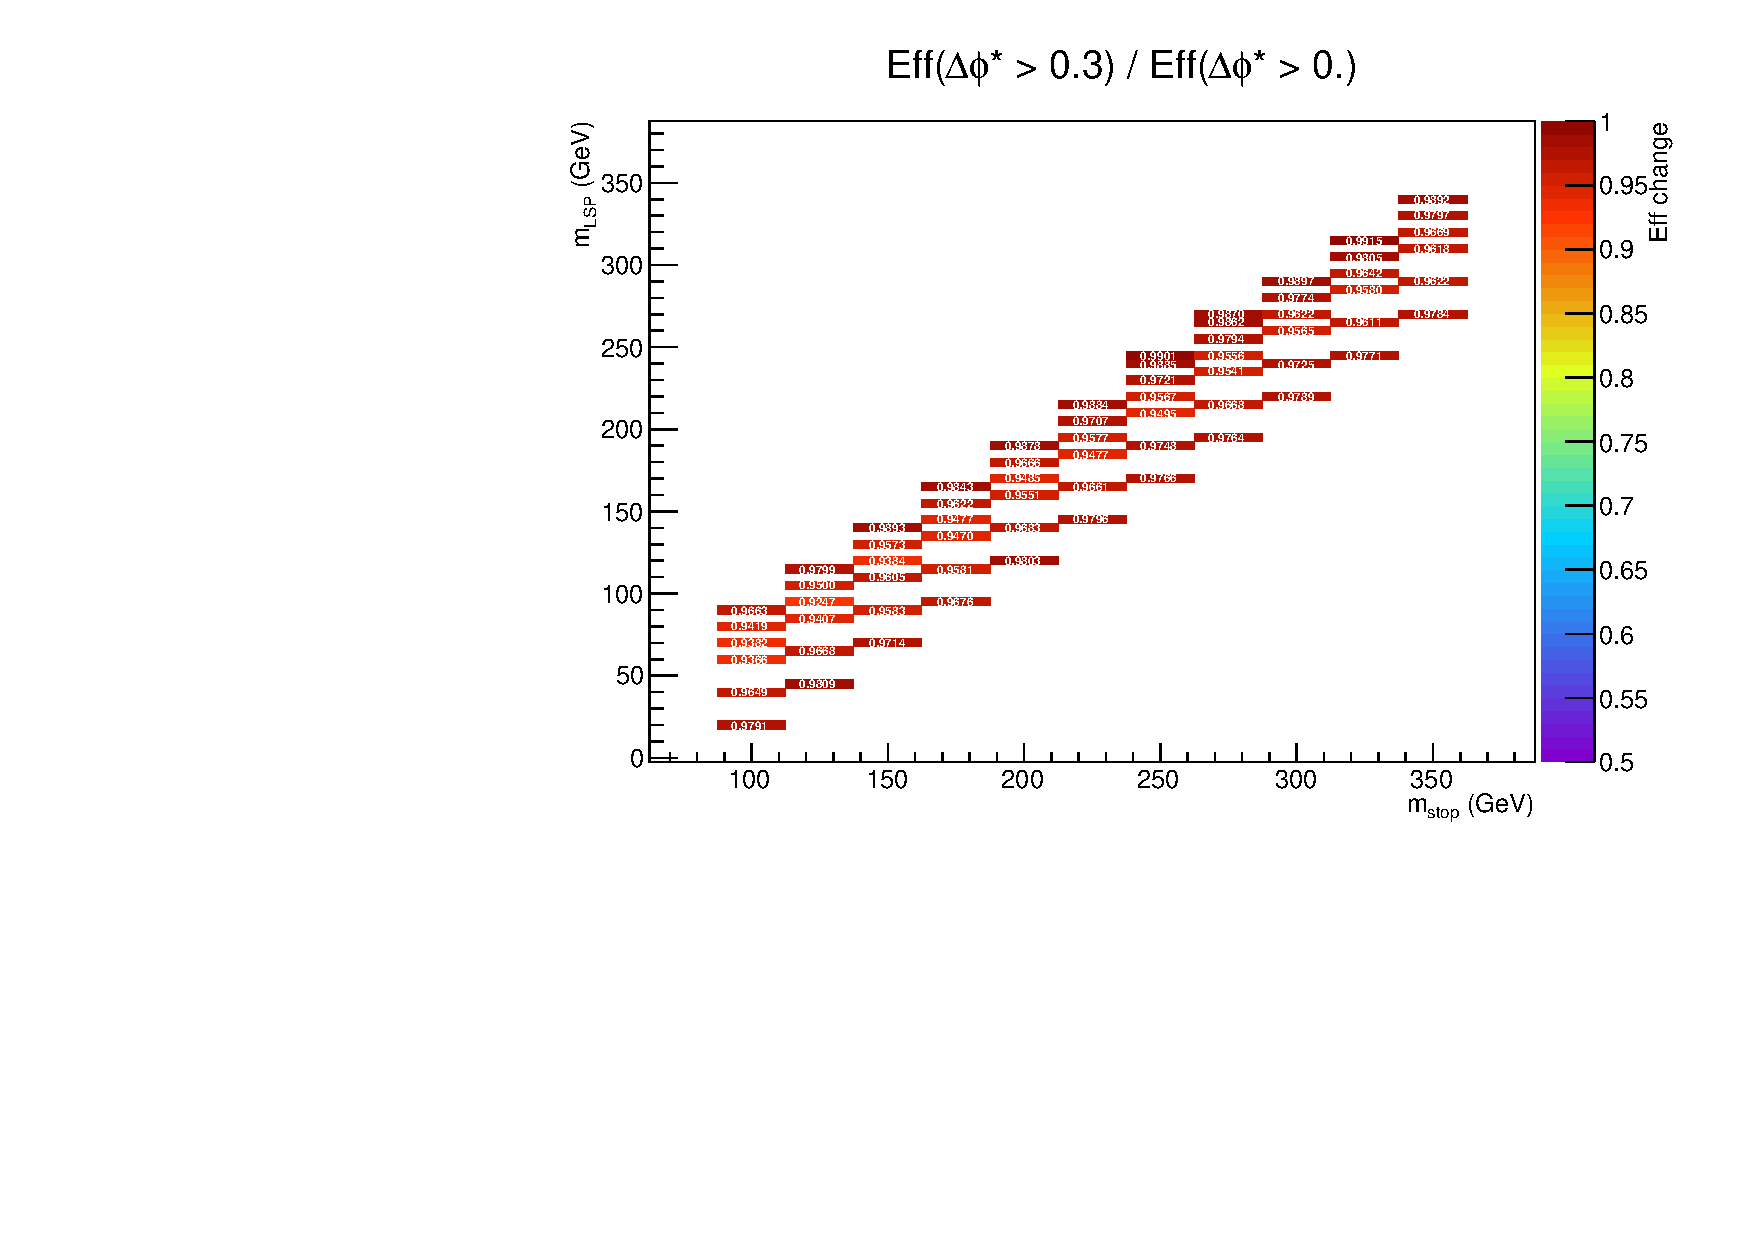
\includegraphics[width=\textwidth]
    {Figs/sms/t2cc/v37/eff_changes/eff_compare_2d_T2cc_v37_vs_T2cc_v38_eq0b_le3j}
    \caption{\njlow, $\nb = 0$}
    \label{fig:t2cc_dphistar_eq0b_le3j}
  \end{subfigure}
  \begin{subfigure}[b]{0.46\textwidth}
    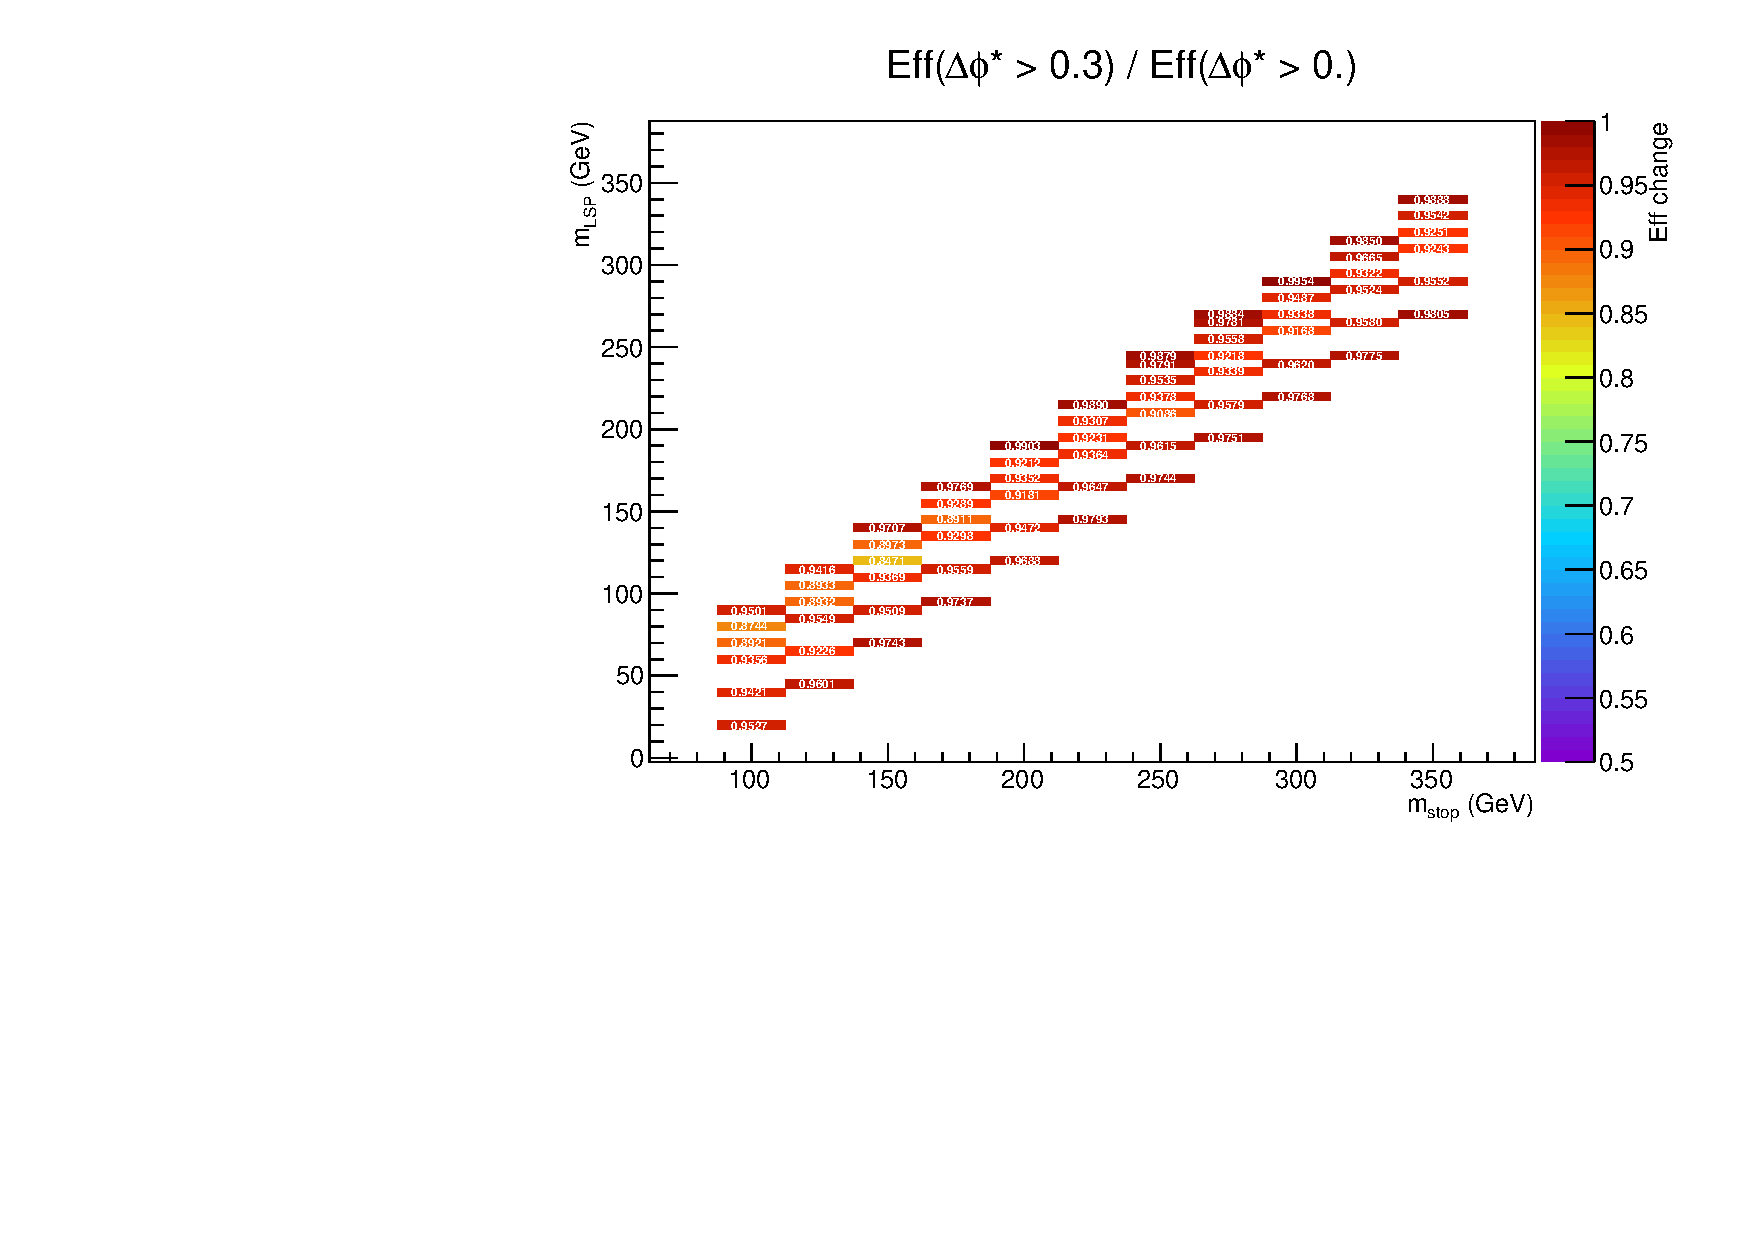
\includegraphics[width=\textwidth]
    {Figs/sms/t2cc/v37/eff_changes/eff_compare_2d_T2cc_v37_vs_T2cc_v38_eq1b_le3j}
    \caption{\njlow, $\nb = 1$}
    \label{fig:t2cc_dphistar_eq1b_le3j}
  \end{subfigure}\\
  \vspace{0.2cm}
  \begin{subfigure}[b]{0.46\textwidth}
    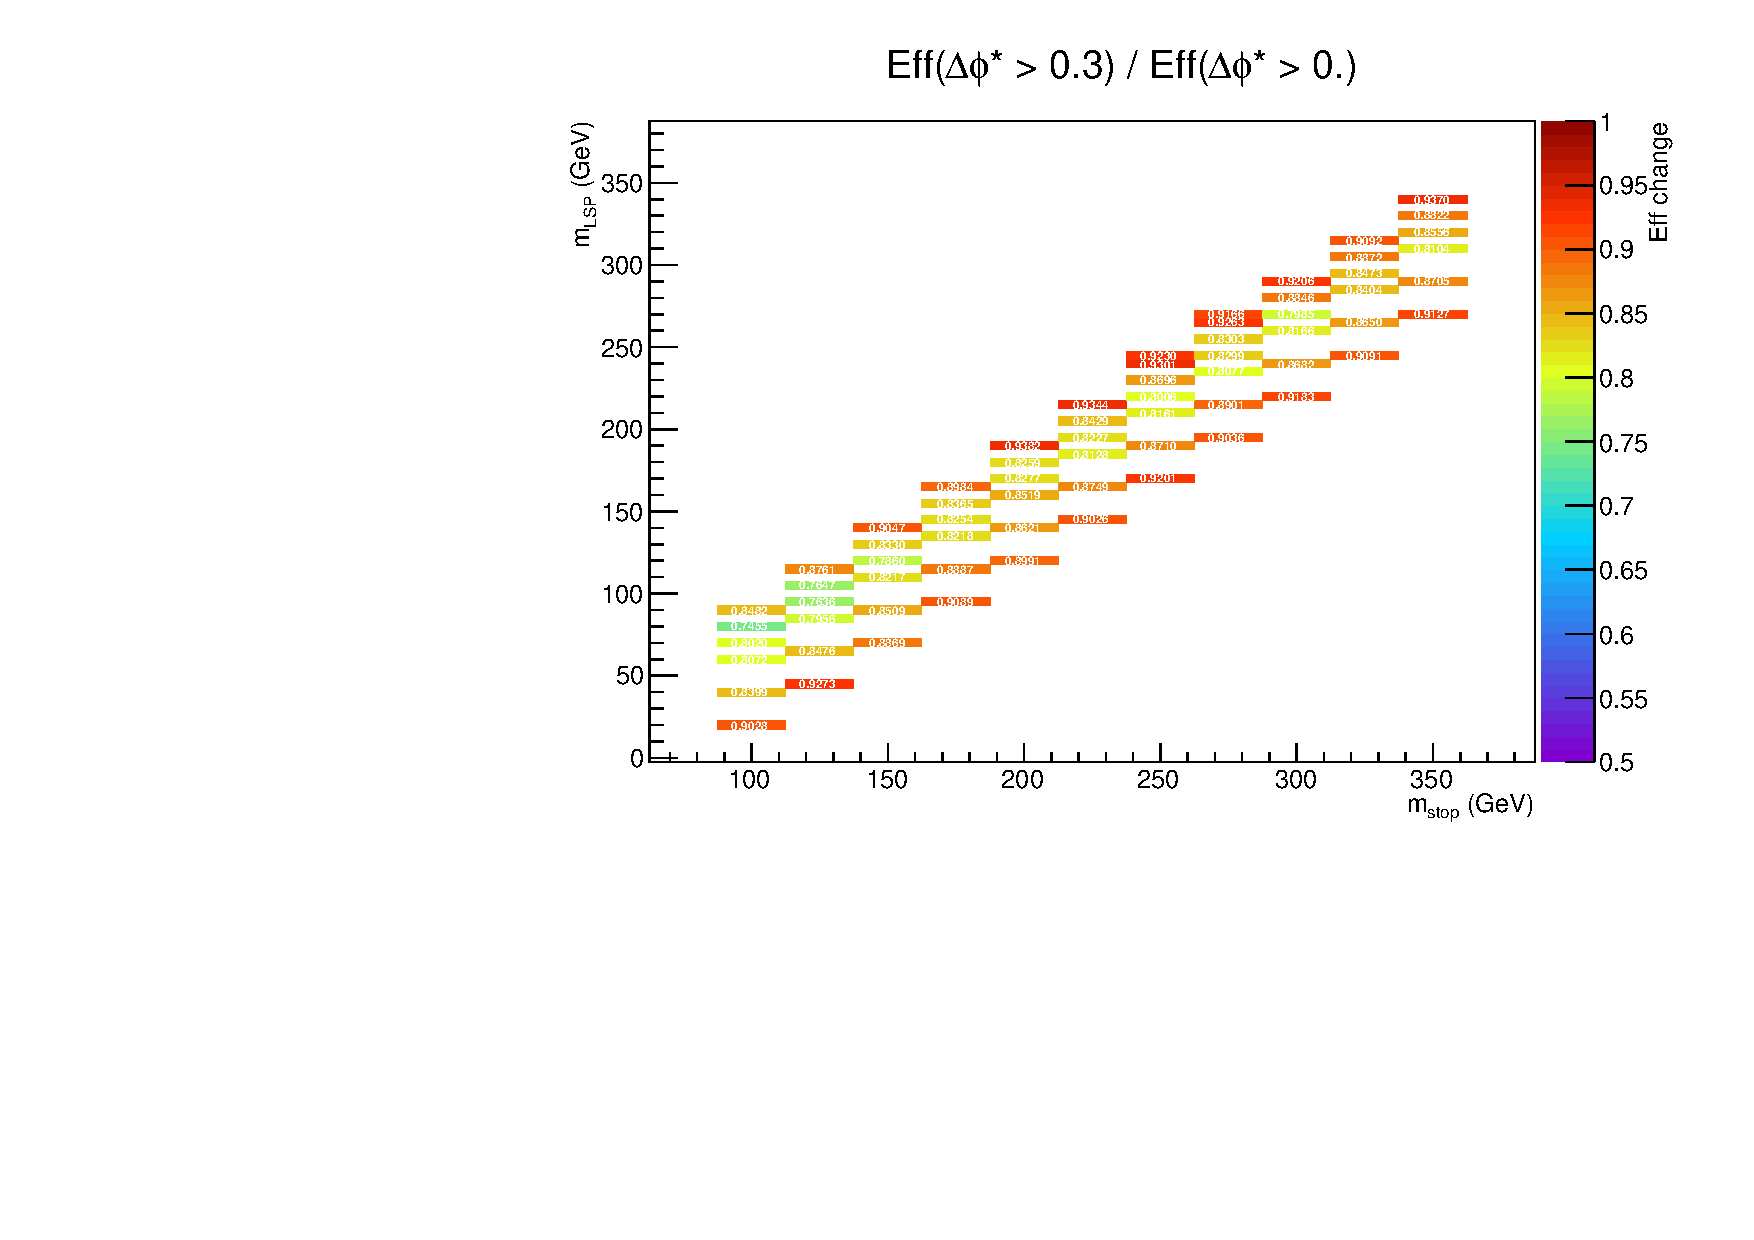
\includegraphics[width=\textwidth]
    {Figs/sms/t2cc/v37/eff_changes/eff_compare_2d_T2cc_v37_vs_T2cc_v38_eq0b_ge4j}
    \caption{\njhigh, $\nb = 0$}
    \label{fig:t2cc_dphistar_eq0b_ge4j}
  \end{subfigure}
  \begin{subfigure}[b]{0.46\textwidth}
    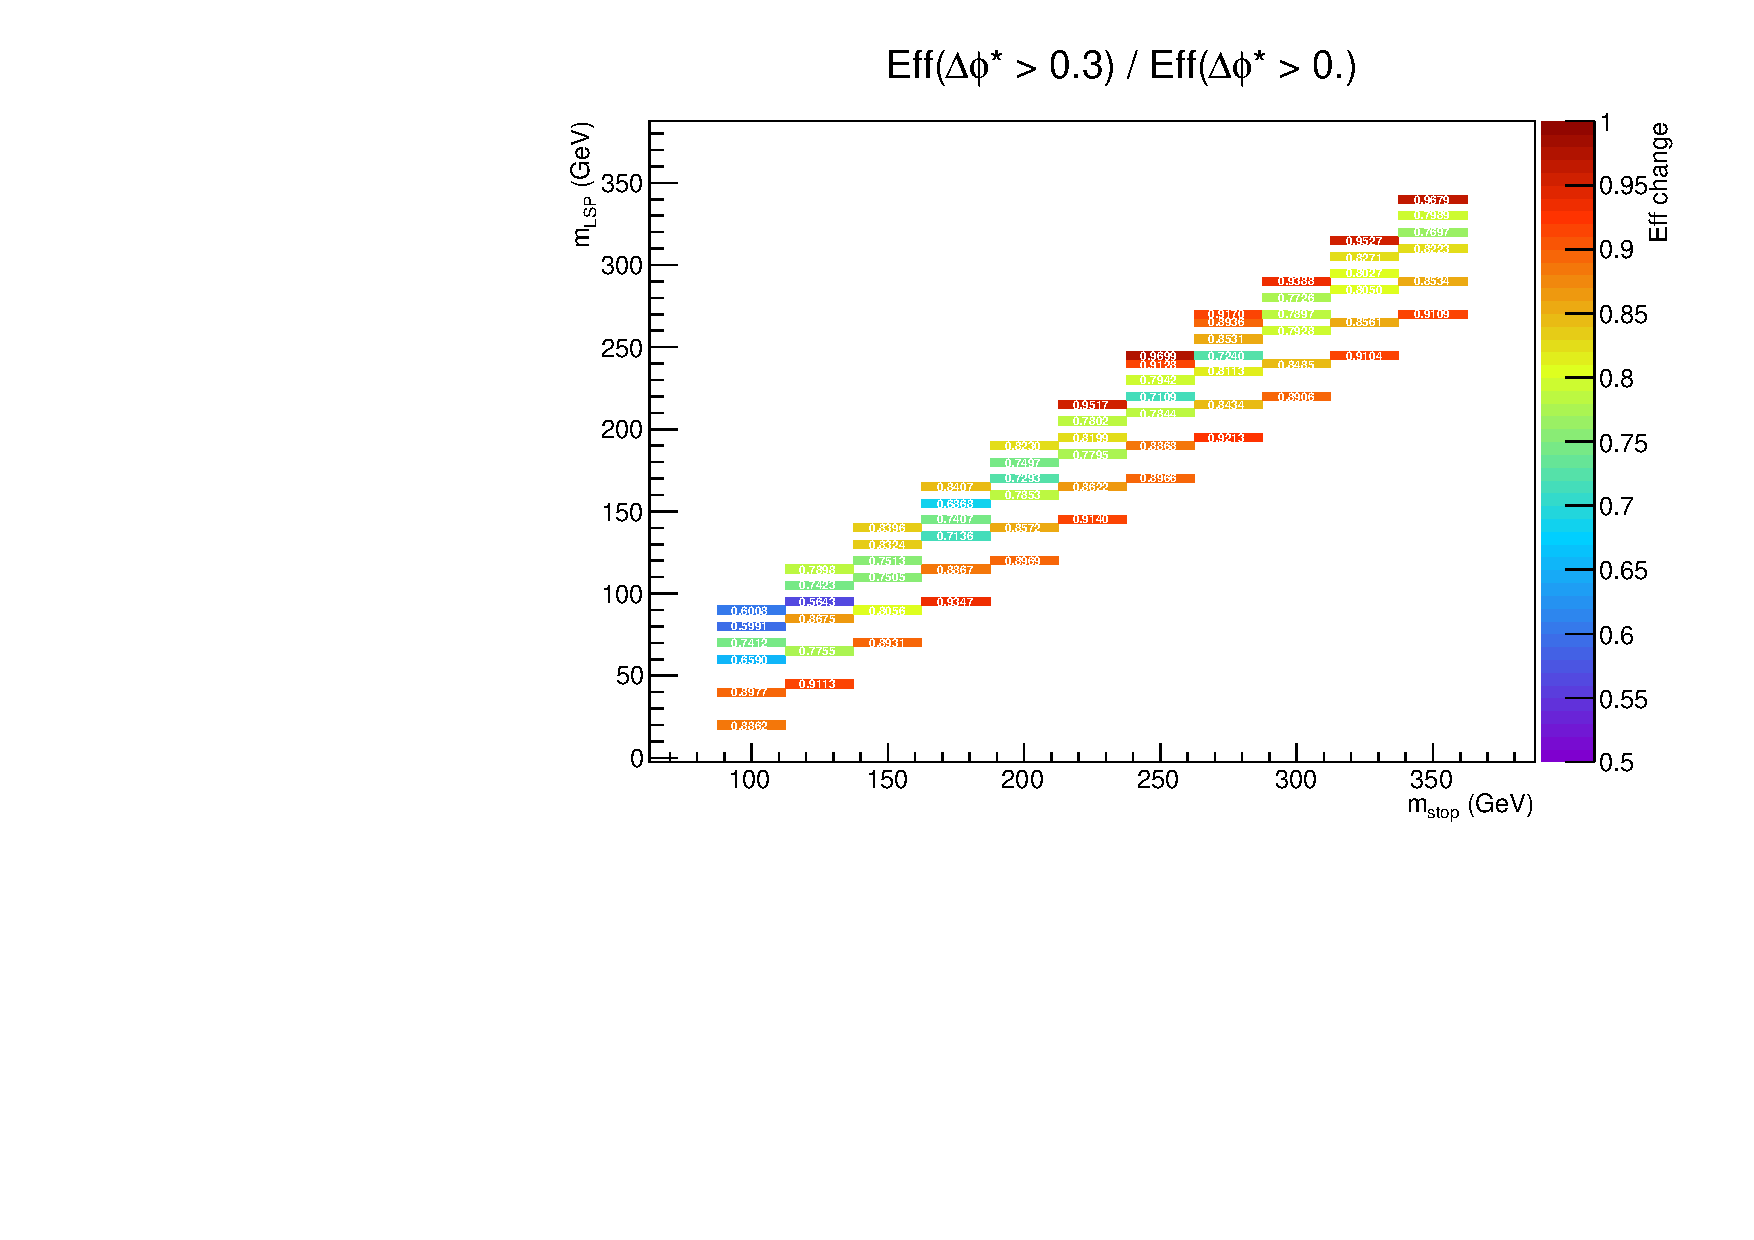
\includegraphics[width=\textwidth]
    {Figs/sms/t2cc/v37/eff_changes/eff_compare_2d_T2cc_v37_vs_T2cc_v38_eq1b_ge4j}
    \caption{\njhigh, $\nb = 1$}
    \label{fig:t2cc_dphistar_eq1b_ge4j}
  \end{subfigure}
  \caption{The change in acceptance of the \texttt{T2cc} model when applying
  the \mindphistar > 0.3 requirement. Plots are shown for the four relevant
  categories used for interpretation, with an inclusive selection of \HT > 200
  \gev}
  \label{fig:t2cc_dphistar_effchange}
\end{figure}

\begin{figure}[h!]
  \centering
  \begin{subfigure}[b]{0.46\textwidth}
    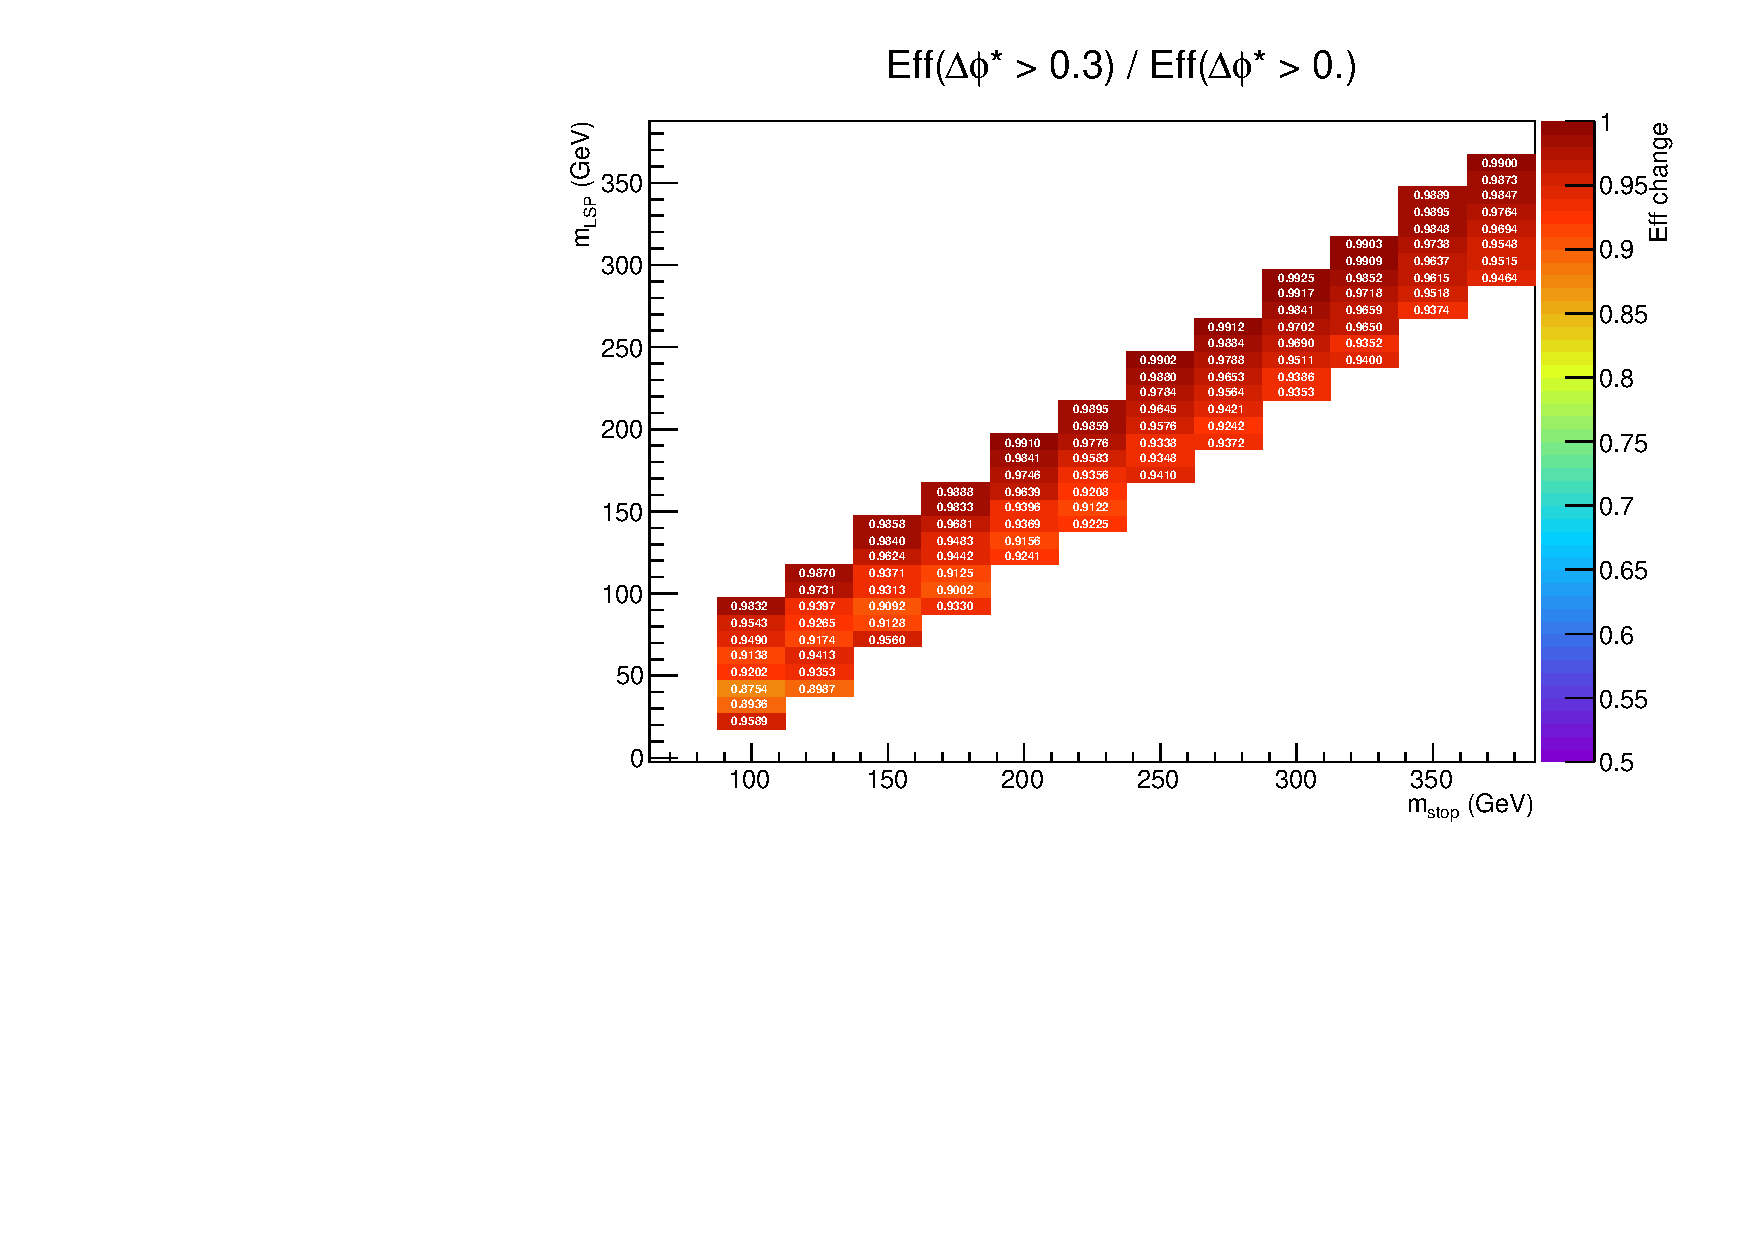
\includegraphics[width=\textwidth]
    {Figs/sms/t2degen/v19/eff_changes/eff_compare_2d_T2_4body_v19_vs_T2_4body_v20_eq0b_le3j}
    \caption{\njlow, $\nb = 0$}
    \label{fig:t2degen_dphistar_eq0b_le3j}
  \end{subfigure}
  \begin{subfigure}[b]{0.46\textwidth}
    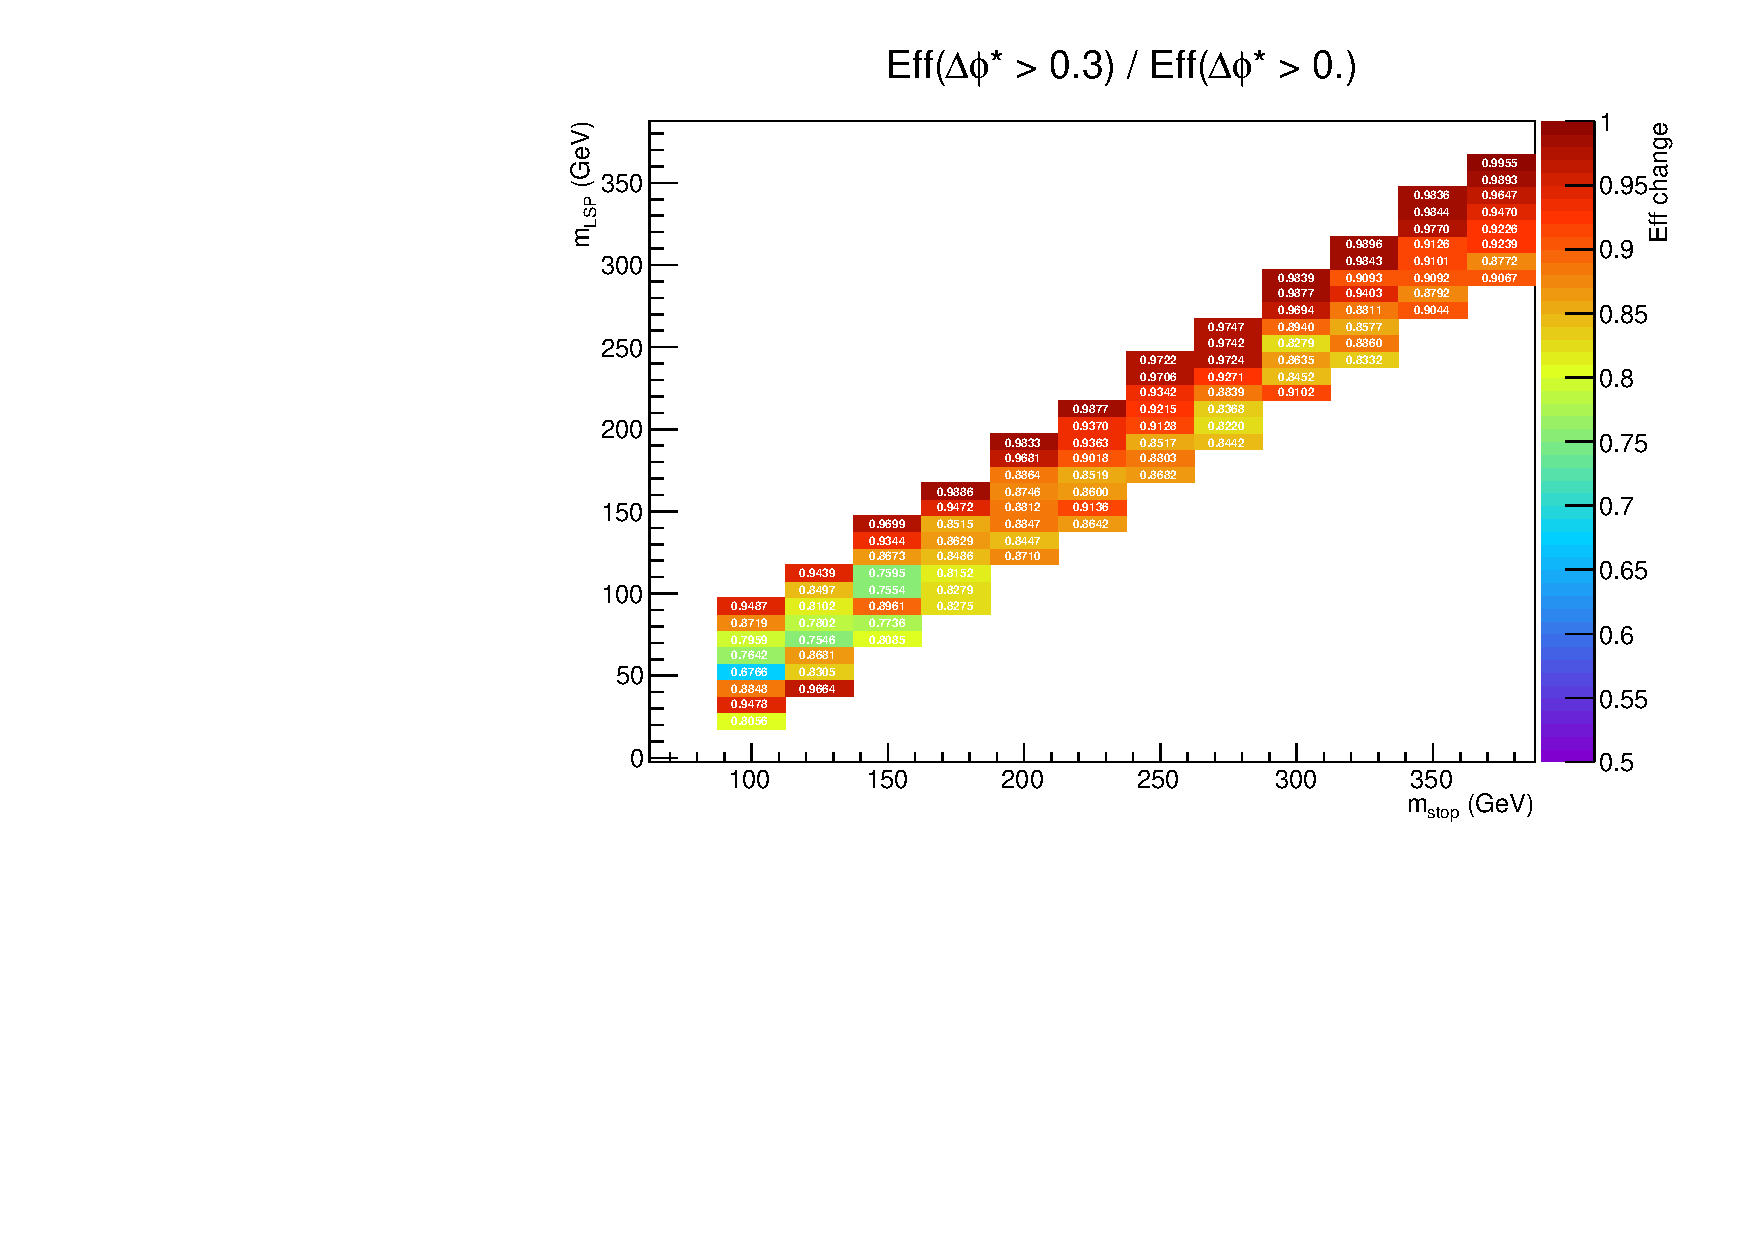
\includegraphics[width=\textwidth]
    {Figs/sms/t2degen/v19/eff_changes/eff_compare_2d_T2_4body_v19_vs_T2_4body_v20_eq1b_le3j}
    \caption{\njlow, $\nb = 1$}
    \label{fig:t2degen_dphistar_eq1b_le3j}
  \end{subfigure}\\
  \vspace{0.2cm}
  \begin{subfigure}[b]{0.46\textwidth}
    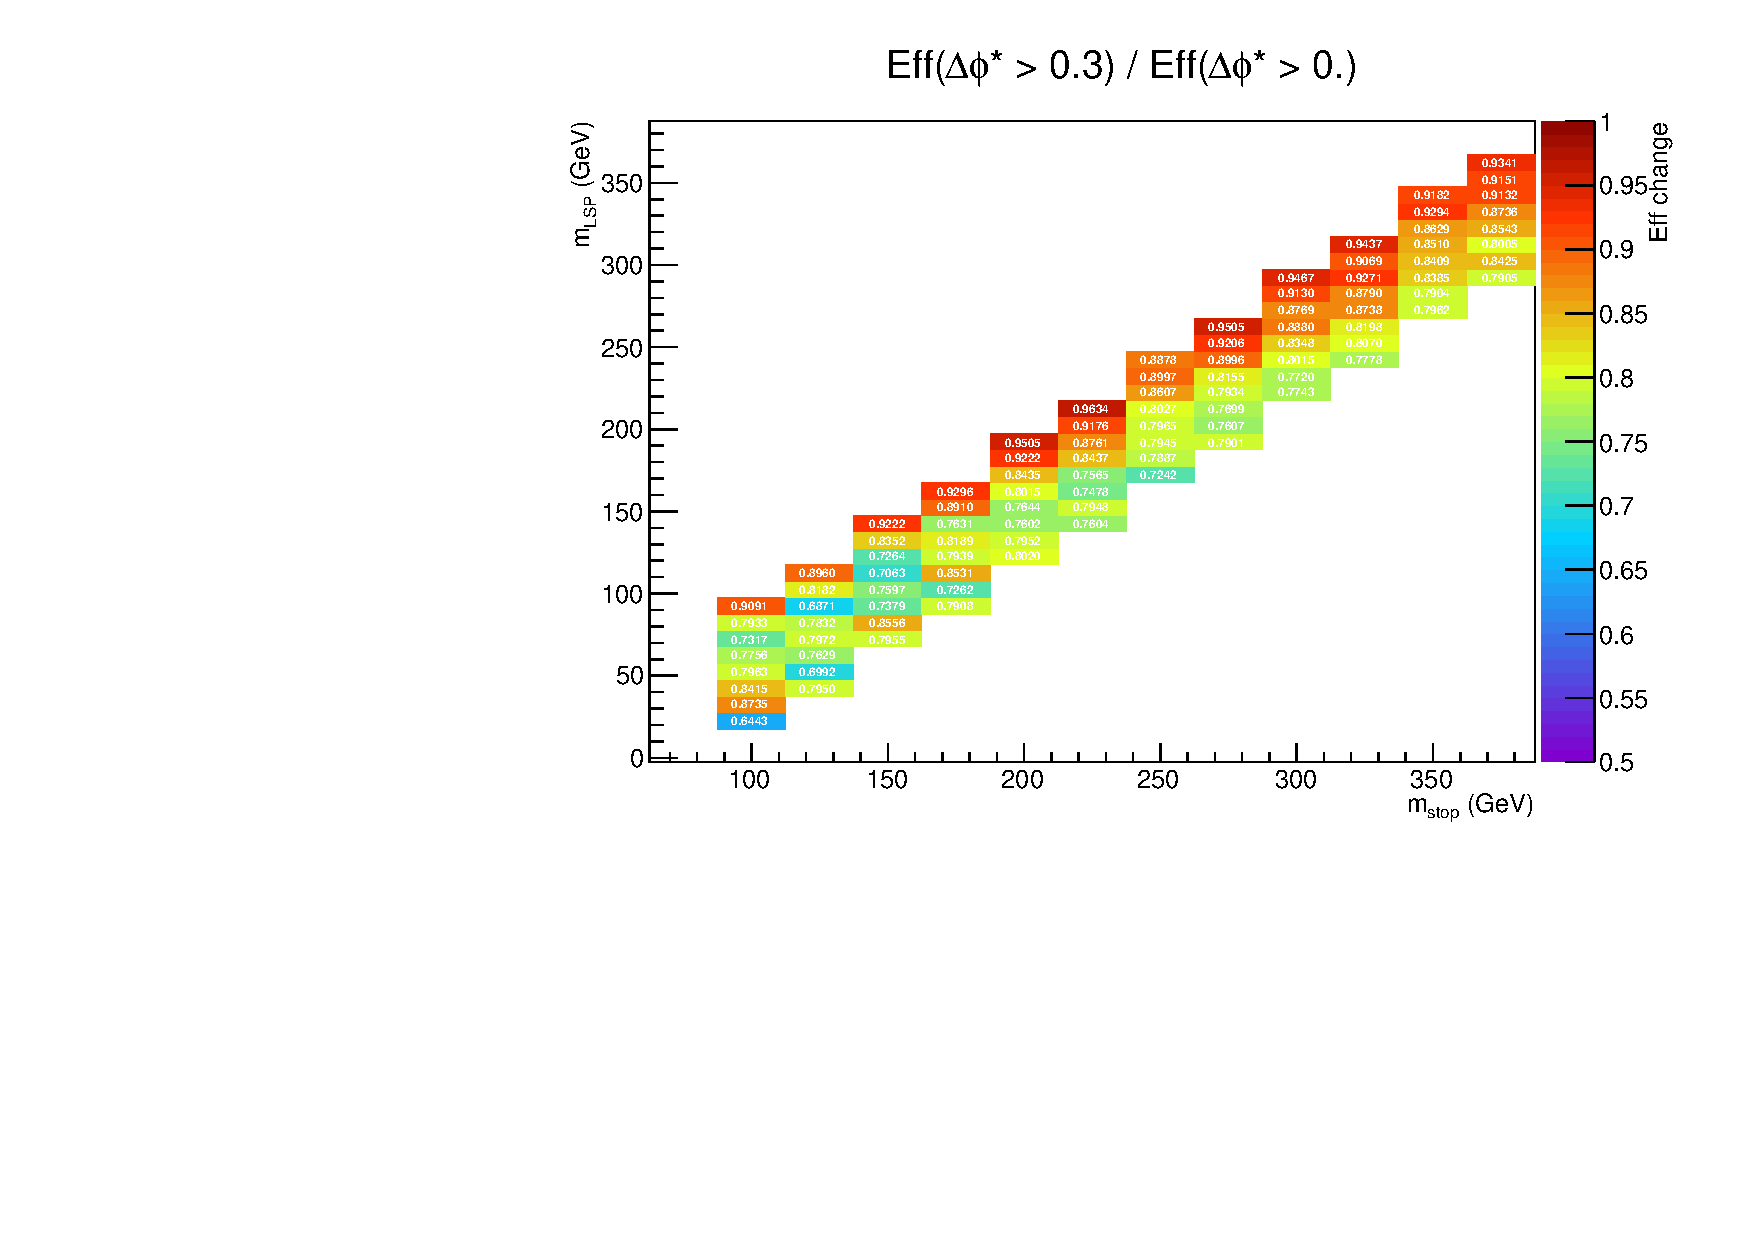
\includegraphics[width=\textwidth]
    {Figs/sms/t2degen/v19/eff_changes/eff_compare_2d_T2_4body_v19_vs_T2_4body_v20_eq0b_ge4j}
    \caption{\njhigh, $\nb = 0$}
    \label{fig:t2degen_dphistar_eq0b_ge4j}
  \end{subfigure}
  \begin{subfigure}[b]{0.46\textwidth}
    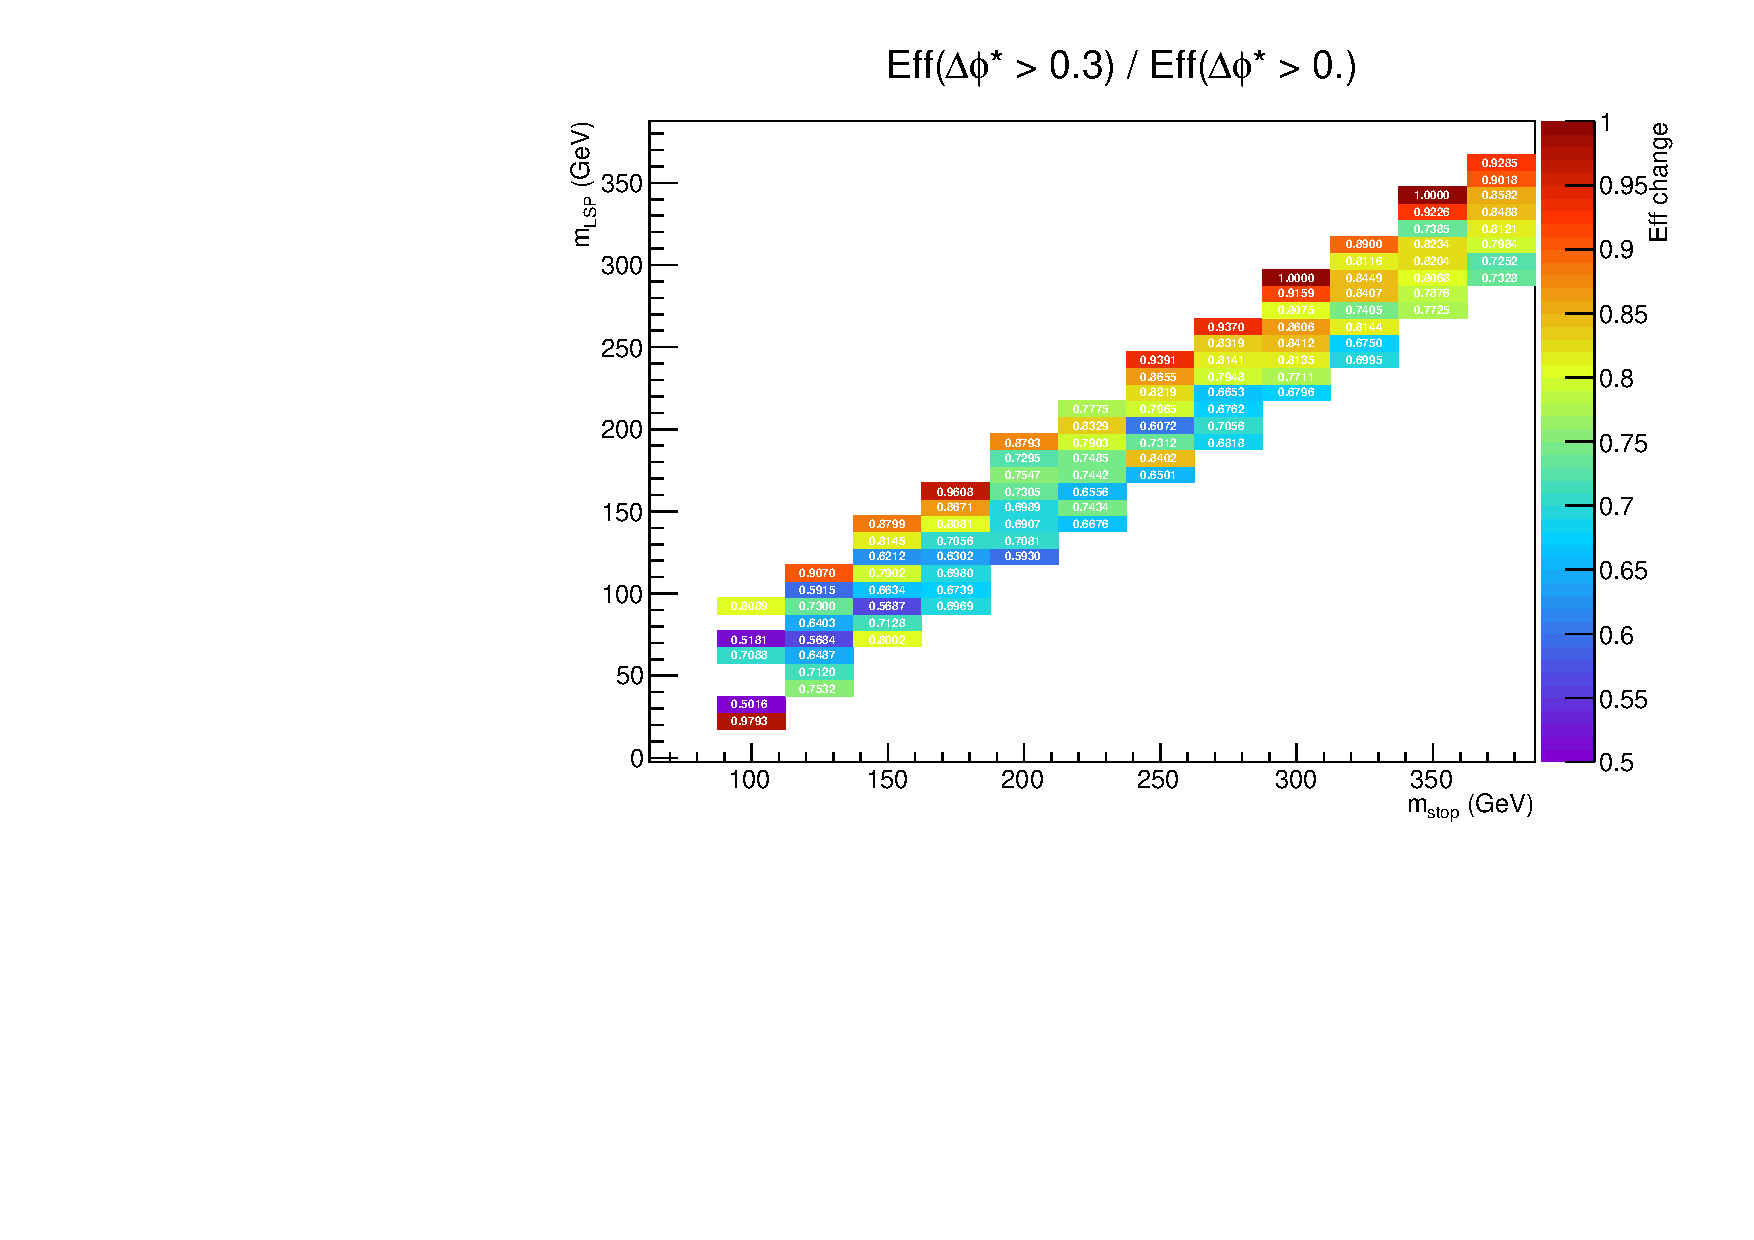
\includegraphics[width=\textwidth]
    {Figs/sms/t2degen/v19/eff_changes/eff_compare_2d_T2_4body_v19_vs_T2_4body_v20_eq1b_ge4j}
    \caption{\njhigh, $\nb = 1$}
    \label{fig:t2degen_dphistar_eq1b_ge4j}
  \end{subfigure}
  \caption{The change in acceptance of the \texttt{T2degen} model when applying
  the \mindphistar > 0.3 requirement. Plots are shown for the four relevant
  categories used for interpretation, with an inclusive selection of \HT > 200
  \gev}
  \label{fig:t2degen_dphistar_effchange}
\end{figure}

Model acceptance change due to the requirement appears to be intrinsically
linked to the mutliplicity of objects, in this case jets, in the event. The
\njhigh categories appear to reduce acceptance the most. A similar trend is
seen when going from \nb = 0 to \nb = 1, most noticably in \texttt{T2degen},
where the b-tagged jet will predominantly come from the real b-quark in the
decay. The configuration of a boosted SUSY decay system containing both jets and
invisible \chiz particles could have appear like the heavy flavour QCD events
this cut is targetted at removing. 

Additionally an increased number of jets in the event, as seen in the higher \nj
category, increases the probability of a jet mis-measurement which could lead to
low values of \mindphistar, thus causing an event to be removed.

\clearpage
\begin{sidewaysfigure}
    \centering
    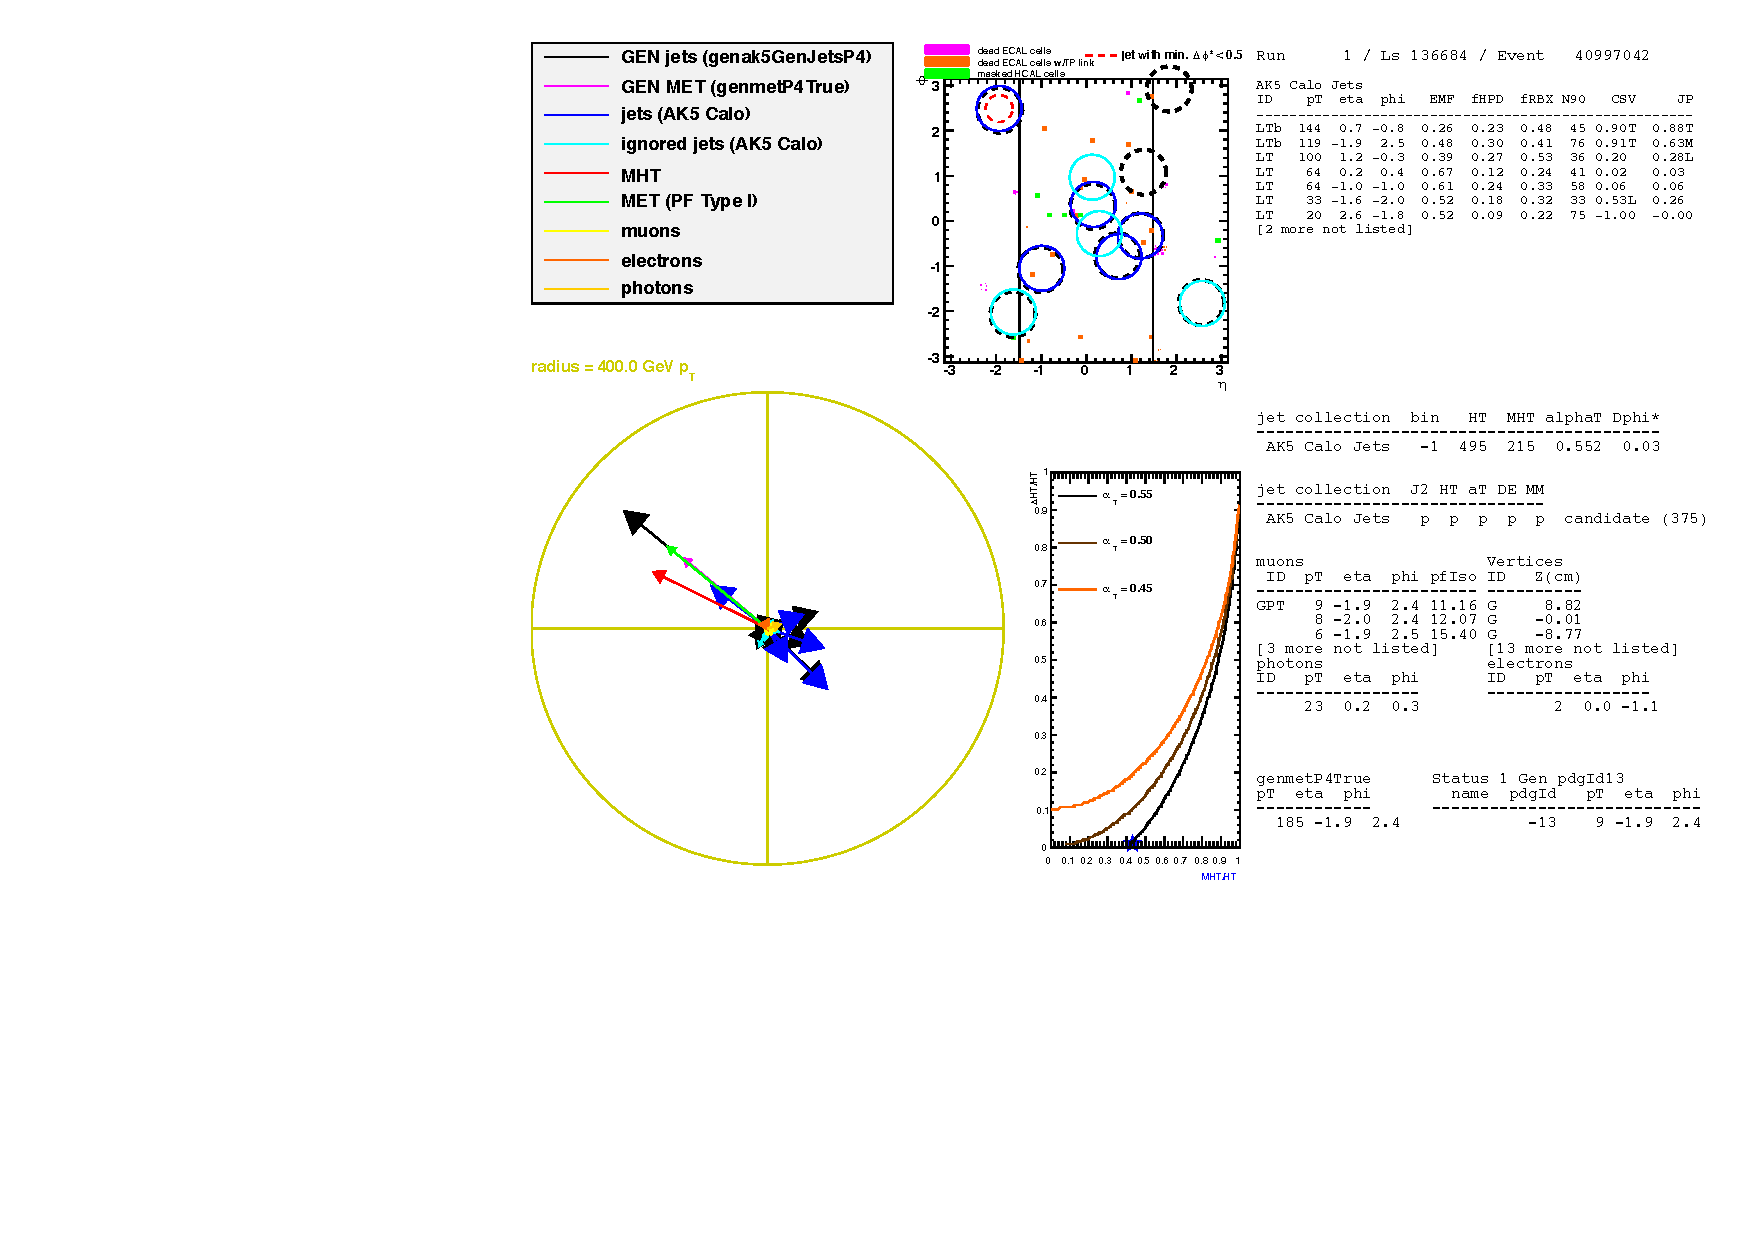
\includegraphics[width=0.95\textwidth]
    {Figs/eventDisplays/Had_QCD_MG_MC_HT375_skim_displays_singleEvent_2_noPF.pdf}
    \caption{An event display of a typical heavy flavour QCD event, with a jet
    decaying leptonically with high-\Pt neutrinos and therefore considerable
    generator-level \met.}
    \label{fig:event_display_QCD}
\end{sidewaysfigure}
